
\subsection{Get the network} 

To get the data for our simulation, we used the so-called Facebook Graph API, a programming tool designed to support better access to conventions on the facebook social media platform.\footnote{http://www.techopedia.com/definition/28984/facebook-graph-api} Unfortunately, there is no implementation for MATLAB, so the data-fechting was programmed in python using facebook sdk.\footnote{https://github.com/pythonforfacebook/facebook-sdk} 

\paragraph{Get access}

First, one needs to get access to the social graph. Therefore, an access token is required.\footnote{https://developers.facebook.com/docs/facebook-login/access-tokens/}



\paragraph{Get graph}

Having enterd a valid token, one can access all information this token provides.  For simplicty, only the non-anonymized case is discussed in detail (for more details on the anonymization, look at subsection anonymization).

\begin{lstlisting} 
profile = graph.get_object("me")
friends = graph.get_connections("me", "friends")
\end{lstlisting}
\vspace{4mm}

\noindent For this work not only data of ones own profile is of interest, but also all available information one gets from his friends.
The object friends is an array containing all id's and data of the friends. Since the focus of this work does not lie primary on the direct friends, but the connection in between them, we have to access at least the mutual friends. 

\begin{lstlisting}
mutualfriends = graph.get_connections(tfriend, "mutualfriends")
\end{lstlisting}

\paragraph{Get activity}

For each friend the number of posts per day is determined. This ratio indicates the activity of each individual on facebook. 

\paragraph{Get coordinates}
To visualise the network in MATLAB, the software "Gephi" was used to determine the x- and y- coordinates of each individual. Therefore, the file "gephi.csv", an edge list of the network, was imported. The nodes were then arranged in communities using the layout method "ForceAtlas2". Finally, normalised node coordinates where exported to "coordinates.gdf". After deleting all headers and all edge data from this file, the coordinates could be easily imported to MatLab. The Network is visualized in Figure \ref{Network-Graph}.

\begin{figure}
\begin{center}
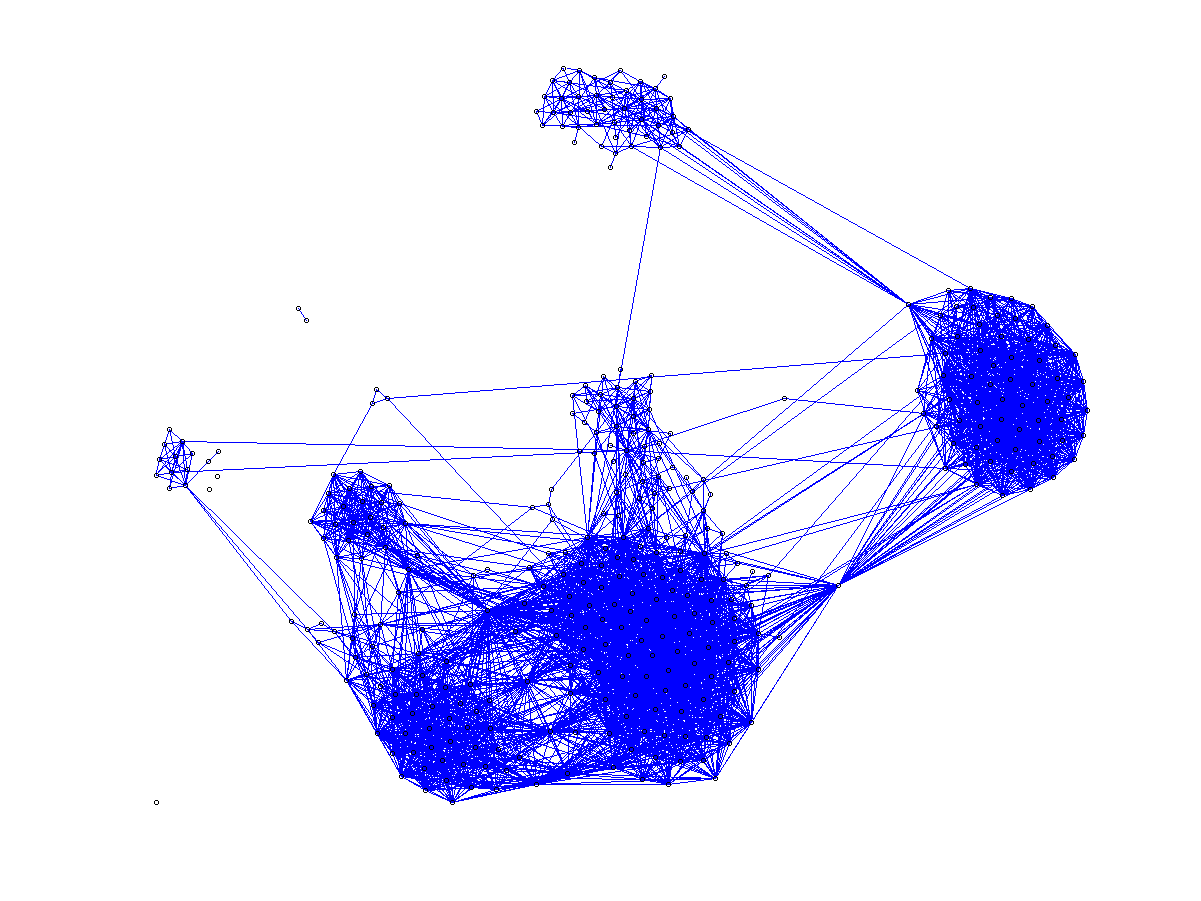
\includegraphics[width=7cm]{Network-Graph}
\caption{A graph of the used facebook network with all edges.}
\label{Network-Graph}
\end{center}
\end{figure}

\paragraph{Anonymisation}

The anonymisation is acutally only a pseudo-anonymisation. First all id's get arranged in order of size. Secondly, a list from 1 to n (number of friends) is created. One then defines a bijection between the two sets, such that the i-th element of the first set, maps to the i-th element of the second set. Even though, this is not really anonymising our data. It is more then sufficient for our purpose, the privacy.



\clearpage
